\documentclass[svgnames,11pt]{beamer}
\input{/home/tof/Documents/Cozy/latex-include/preambule_commun.tex}
\input{/home/tof/Documents/Cozy/latex-include/preambule_beamer.tex}
%\usepackage{pgfpages} \setbeameroption{show notes on second screen=left}
\author[]{Christophe Viroulaud}
\title{Applications Android\\
Données en table}
\date{\framebox{\textbf{Tab 01}}}
%\logo{}
\institute{Première - NSI}
%DODO modifier (encoding="utf8")+ revoir la partie traitement (P30 environ) + enlever les "NaN"
\begin{document}

\begin{frame}
    \titlepage
    \note{\fcolorbox{black}{red}{{\LARGE googleplaystore.zip sur site}}

        googleplaystore.csv, specifications-app.csv, notes.csv}
\end{frame}

\begin{frame}
    \begin{center}
        \centering
        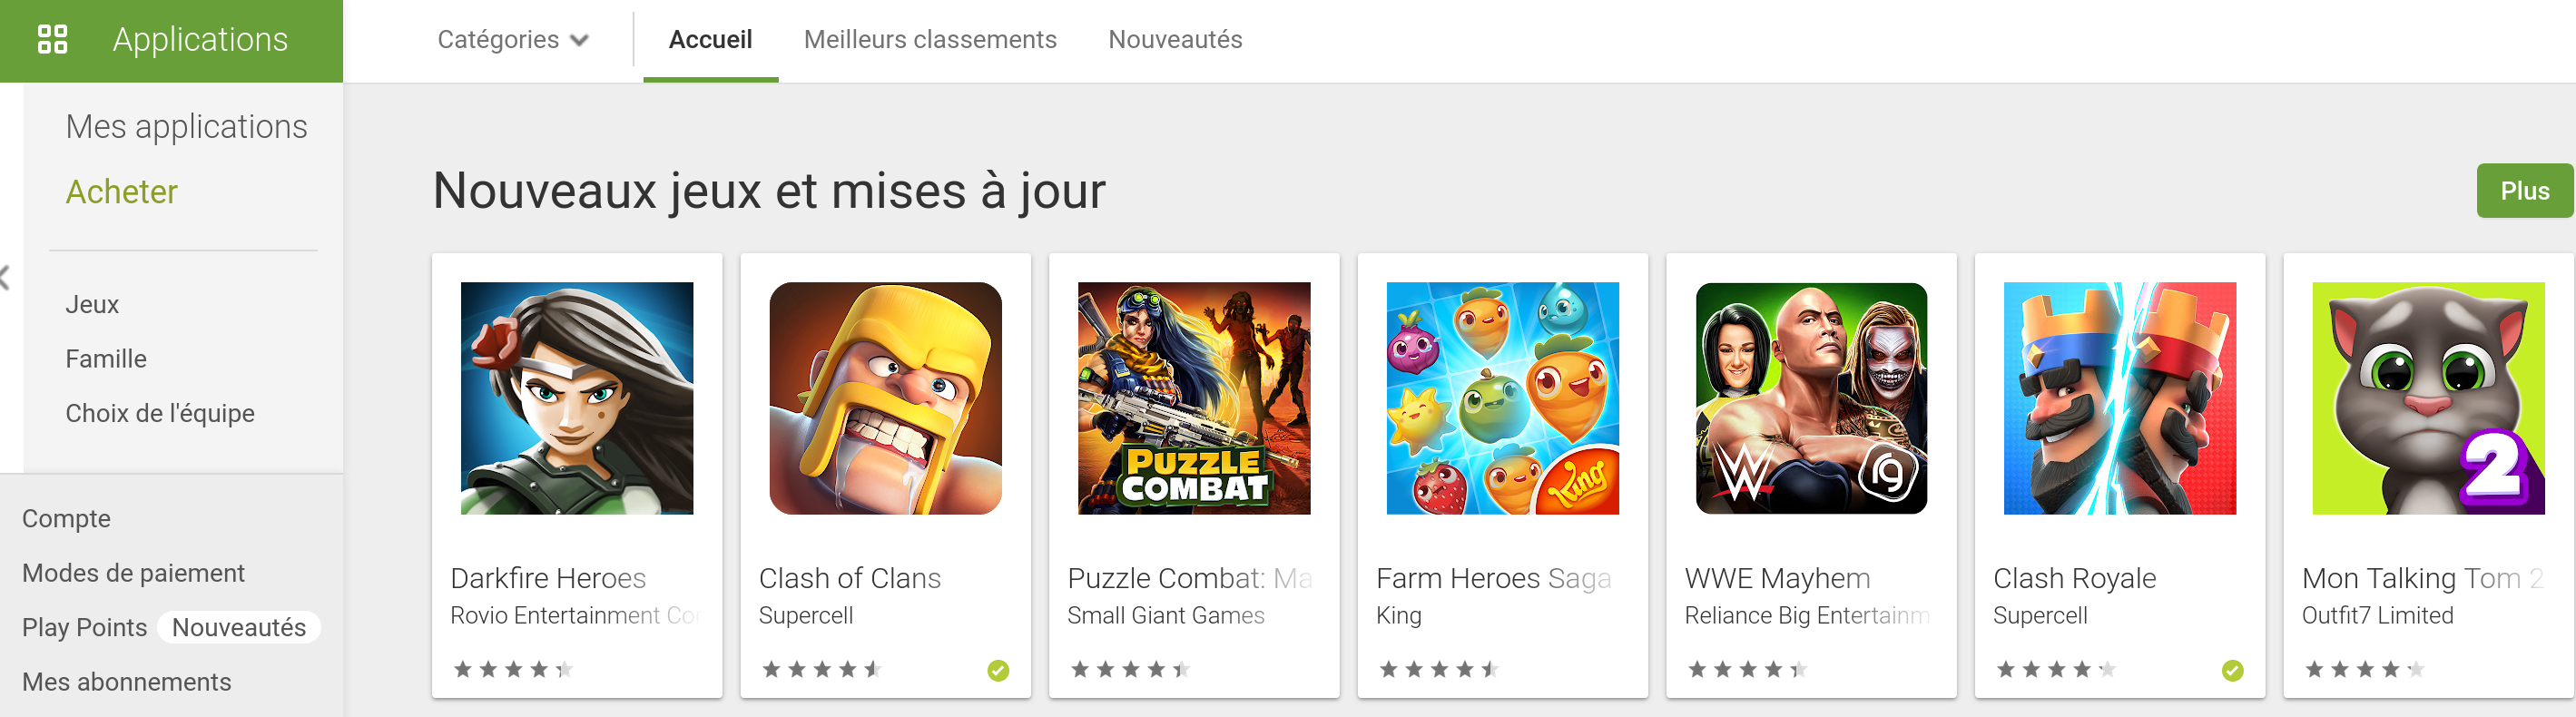
\includegraphics[width=8cm]{ressources/playstore.png}
        \captionof{figure}{Magasin d'applications}
        \label{IMG}
    \end{center}
    \begin{center}
        Chaque carte contient plusieurs informations:
        \begin{itemize}
            \item nom
            \item description
            \item note
            \item image
            \item \dots
        \end{itemize}
    \end{center}
\end{frame}

\begin{frame}
    \begin{center}
        \centering
        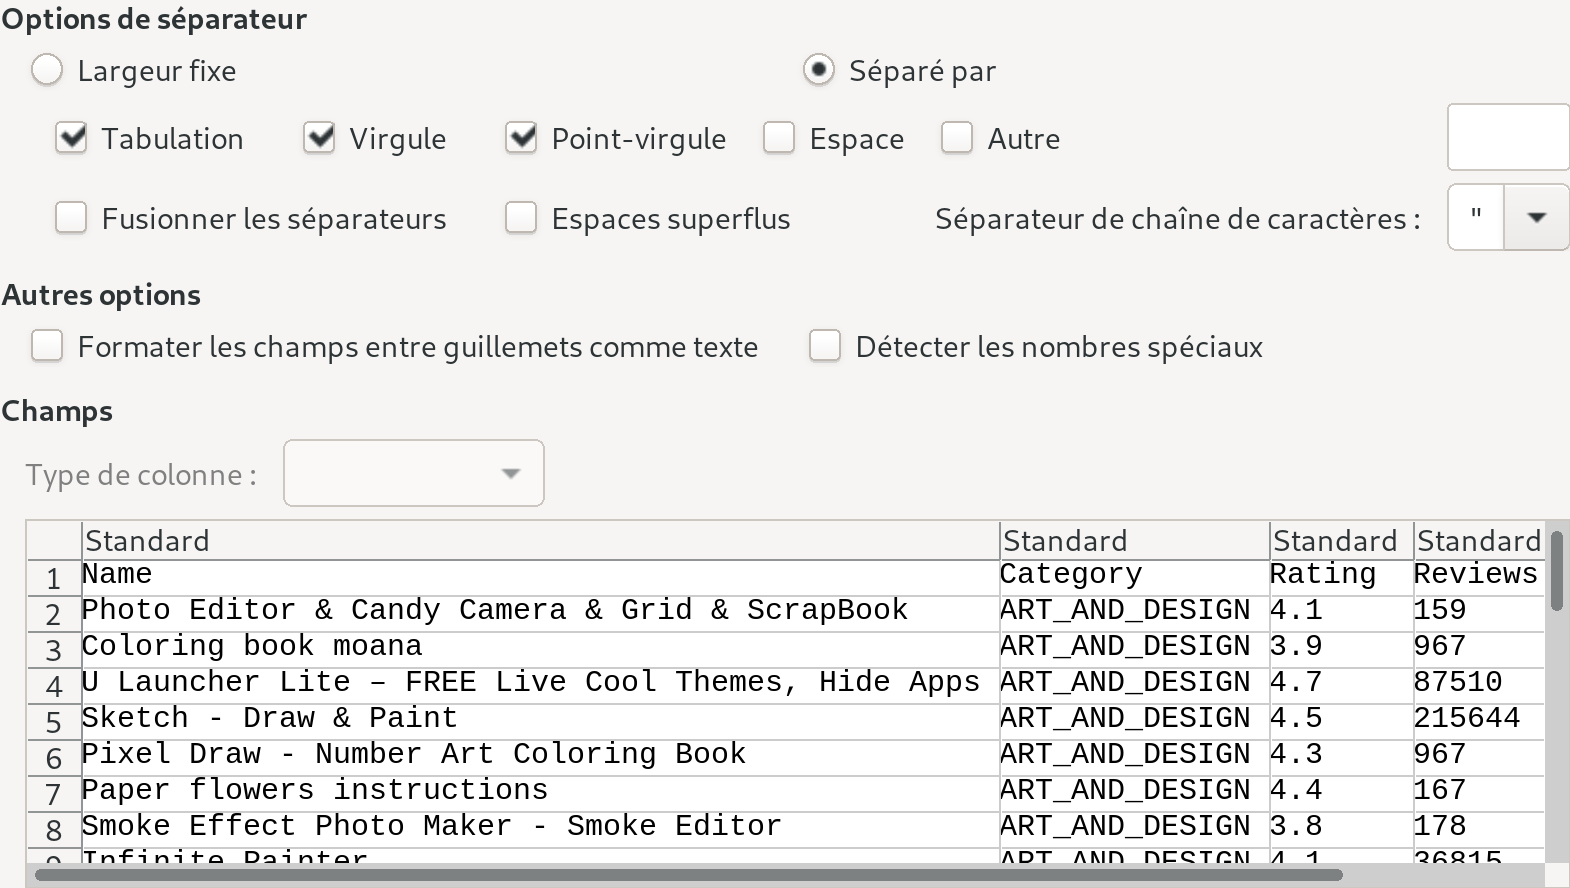
\includegraphics[width=8cm]{ressources/jeu-donnees.png}
        \captionof{figure}{Données stockées dans un fichier texte}
        \label{IMG}
    \end{center}
    \begin{framed}
        \centering Comment manipuler un jeu de données par programmation?
    \end{framed}

\end{frame}
\section{Données en table}
\subsection{Présentation}
\begin{frame}
    \frametitle{Données en table - présentation}

    \note{terme BDD: entité, table (ou relation), attributs}
    \begin{aretenir}[]
        Un fichier de données regroupe des informations organisées.\\Dans un fichier \textbf{\texttt{csv (Comma Separated Values)}}, chaque ligne représente une nouvelle \textbf{entité} du jeu de données. Les informations sont séparées par une virgule, un point-virgule, une tabulation\dots
    \end{aretenir}

\end{frame}
\begin{frame}
    \frametitle{}

    \begin{activite}
        \begin{enumerate}
            \item Télécharger et décompresser l'annexe \textbf{\texttt{app-android.zip}} sur le site \url{https://cviroulaud.github.io}
            \item Avec le \underline{bloc-notes de Windows} ouvrir le fichier \textbf{\texttt{notes.csv}}
            \item Ouvrir le logiciel \emph{LibreOffice Calc}.
            \item Depuis ce logiciel, ouvrir à nouveau le fichier \textbf{\texttt{notes.csv}}
        \end{enumerate}
    \end{activite}

\end{frame}
\begin{frame}
    \frametitle{}

    \begin{center}
        \begin{tabular}{*{3}{c}}
            \hline
            "Nom",         & "Prénom", & "Moyenne" \\
            "Turing" ,     & "Alan" ,  & "19"      \\
            "Von Neuman" , & "John",   & "18"      \\
            "Dijkstra"  ,  & "Edsger", & "17.5"    \\
            "Church"   ,   & "Alonso", & "19"      \\
            \hline
        \end{tabular}
        \captionof{table}{Chaque ligne représente une nouvelle entité}
    \end{center}

\end{frame}
\begin{frame}
    \frametitle{}

    \begin{center}
        \centering
        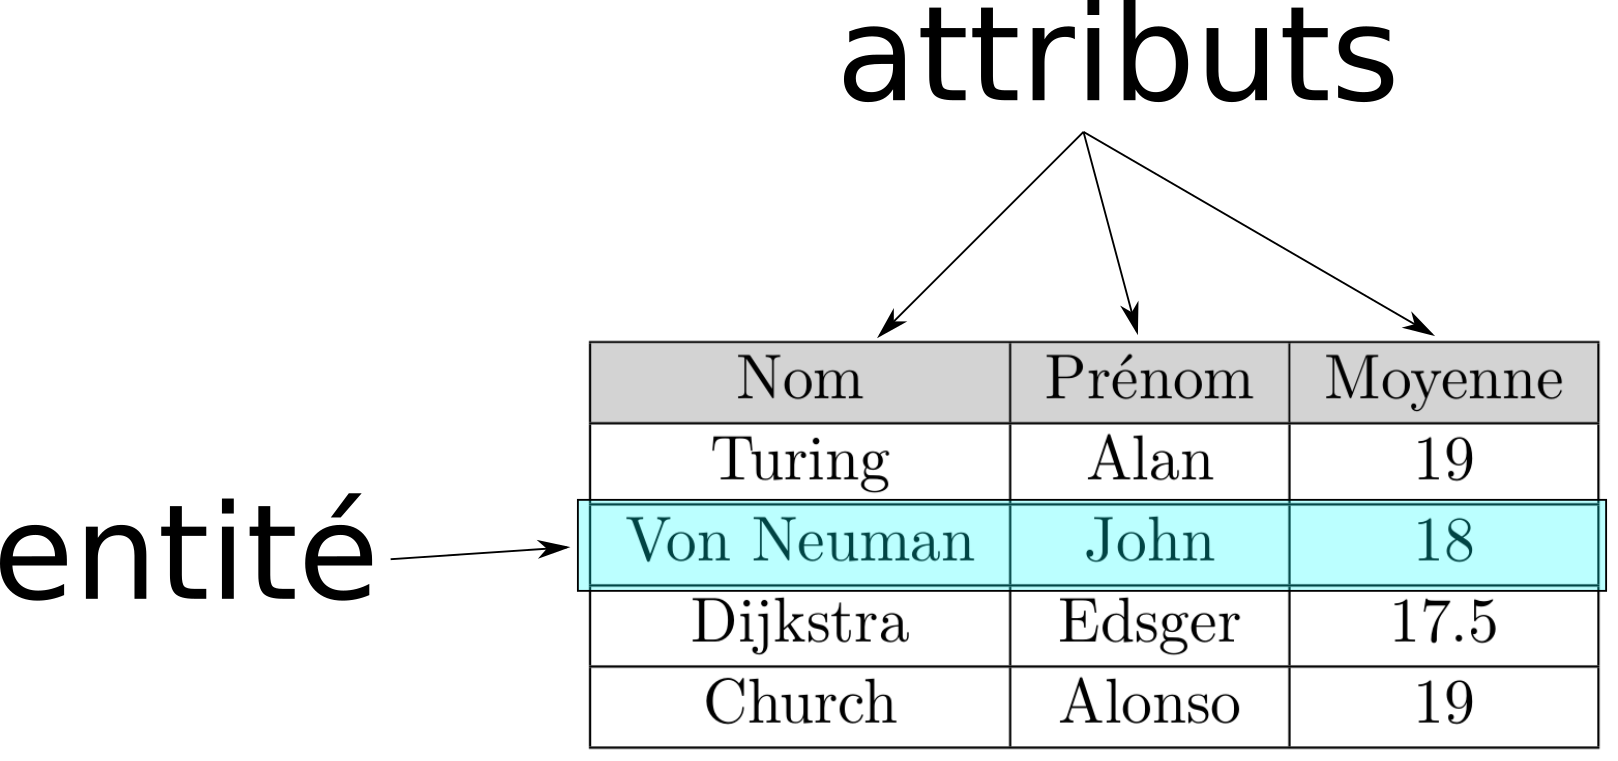
\includegraphics[width=8cm]{ressources/vocabulaire-legende.png}
        \captionof{figure}{LibreOffice reconnaît les fichiers \textbf{\texttt{csv}}}
        \label{IMG}
    \end{center}
    \begin{aretenir}[]
        Un \textbf{attribut} identifie les données d'une même colonne.
    \end{aretenir}

\end{frame}
\begin{frame}
    \frametitle{}

    \begin{activite}
        \begin{enumerate}
            \item Ouvrir le fichier \textbf{\texttt{googleplaystore.csv}} avec LibreOffice Calc.
            \item Trouver le séparateur utilisé.
            \item Repérer les attributs.
        \end{enumerate}
    \end{activite}

\end{frame}
\begin{frame}

    \begin{center}
        \centering
        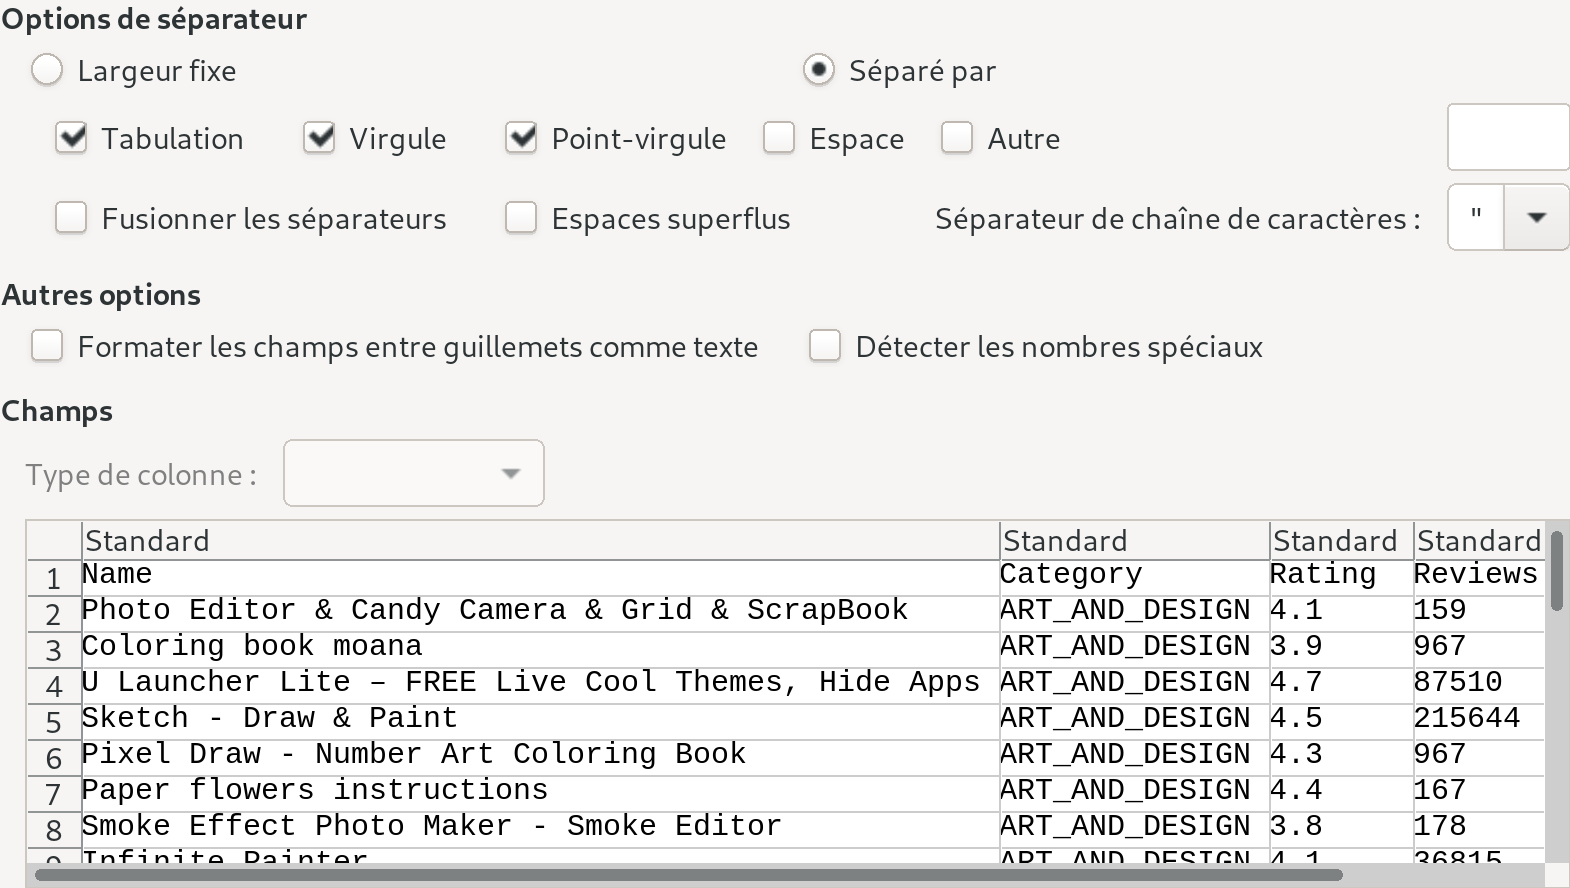
\includegraphics[width=8cm]{ressources/jeu-donnees.png}
        \captionof{figure}{\centering Fichier csv ouvert avec LibreOffice. Le séparateur est la virgule.}
        \label{IMG}
    \end{center}

    \begin{aretenir}[Remarque]
        Quand le nombre de données est important, un tableur est moins approprié pour étudier les données.
    \end{aretenir}
\end{frame}
\begin{frame}

    \begin{itemize}
        \item \emph{Name:} nom,
        \item \emph{Category:} catégorie d'application,
        \item \emph{Rating:} note (sur 5),
        \item \emph{Reviews:} nombre de commentaires,
        \item \emph{Installs:} nombre d'installations.

    \end{itemize}
    \begin{aretenir}[Remarque]
        Chaque ligne représente une application Android
    \end{aretenir}
\end{frame}
\subsection{Lire un fichier avec Python}
\begin{frame}
    \frametitle{Lire un fichier avec Python}
    \begin{aretenir}[]
        Un fichier de données est une \textbf{entrée} dans un programme. Quand on ouvre un fichier externe dans un programme, il est verrouillé. Il faut le \underline{libérer} à la fin de l'utilisation.
    \end{aretenir}

\end{frame}
\begin{frame}[fragile]

    \begin{center}
        \begin{lstlisting}[language=Python , basicstyle=\ttfamily\small, xleftmargin=2em, xrightmargin=2em]
# ouvrir le fichier
fichier = open("notes.csv")

# utiliser le fichier

# libérer le fichier
fichier.close()
\end{lstlisting}
        \captionof{code}{Ouvrir et fermer}
        \label{CODE}
    \end{center}
\end{frame}
\begin{frame}[fragile]
    \frametitle{}

    \begin{activite}
        \begin{enumerate}
            \item Créer le fichier \textbf{\texttt{notes.py}} dans le même dossier que \textbf{\texttt{notes.csv}}
            \item Écrire le code \ref{ouvrir}.
        \end{enumerate}
        \begin{center}
            \begin{lstlisting}[language=Python , basicstyle=\ttfamily\small, xleftmargin=2em, xrightmargin=2em]
# ouvrir le fichier
fichier = open("notes.csv")

# utiliser le fichier

# libérer le fichier
fichier.close()
\end{lstlisting}
            \captionof{code}{Ouvrir et fermer}
            \label{ouvrir}
        \end{center}
    \end{activite}

\end{frame}
\begin{frame}[fragile]
    \frametitle{}
    \begin{center}
        \begin{lstlisting}[language=Python , basicstyle=\ttfamily\small, xleftmargin=2em, xrightmargin=2em]
# ouvrir le fichier
with open("notes.csv") as notes:
    # utiliser le fichier

# fermeture automatique
\end{lstlisting}
        \captionof{code}{Autre méthode}
        \label{ouvrir}
    \end{center}

\end{frame}
\subsection{Lire un fichier \textbf{\texttt{csv}} avec Python}
\begin{frame}
    \frametitle{Lire un fichier \textbf{\texttt{csv}} avec Python}
    \begin{aretenir}[]
        Un programme Python peut ouvrir tous types de fichiers externes (image, texte\dots). Il existe de nombreuses bibliothèques adaptées pour chaque type.\\La bibliothèque \textbf{\texttt{csv}} permet de \textbf{lire} ou \textbf{écrire} ligne après ligne dans un fichier \textbf{\texttt{csv}}.
    \end{aretenir}

\end{frame}
\begin{frame}[fragile]


    \begin{activite}
        Tester le code:
        \begin{center}
            \begin{lstlisting}[language=Python , basicstyle=\ttfamily\small, xleftmargin=2em, xrightmargin=2em]
import csv
# ouvrir le fichier
fichier = open("notes.csv")

lecteur = csv.reader(fichier)
for ligne in lecteur:
    print(ligne)

# libérer le fichier
fichier.close()
\end{lstlisting}
        \end{center}
    \end{activite}
\end{frame}
\begin{frame}
    \frametitle{}

    \begin{aretenir}[]
        La méthode \textbf{\texttt{reader}} de la bibliothèque \textbf{\texttt{csv}} est un \textbf{itérateur}. À chaque appel (itération), l'itérateur lit une nouvelle ligne et la renvoie sous forme de tableau.\\
        \underline{Attention:} un itérateur se vide au fur et à mesure. Il ne peut être parcouru qu'une fois.
    \end{aretenir}
    \begin{aretenir}[Remarque]
        La fonction \textbf{\texttt{range}} est un itérateur qui fournit des entiers.
    \end{aretenir}
\end{frame}
\begin{frame}[fragile]
    \frametitle{}

    \begin{aretenir}[Remarque]
        La méthode \textbf{\texttt{reader}} ne distingue pas les attributs.
    \end{aretenir}
    \begin{center}
        \begin{lstlisting}[language=Python , basicstyle=\ttfamily\small, xleftmargin=2em, xrightmargin=2em]
['nom', 'prenom', 'moyennes']
['Turing', 'Alan', '19']
['Von Neuman', 'John', '18']
['Dijkstra', 'Edsger', '17.5']
['Church', 'Alonso', '19'] 
\end{lstlisting}
    \end{center}
\end{frame}
\begin{frame}
    \frametitle{}

    \begin{activite}
        \begin{enumerate}
            \item Remplacer la méthode \textbf{\texttt{reader}} par \textbf{\texttt{DictReader}}.
            \item Observer les objets obtenus.
        \end{enumerate}
    \end{activite}

\end{frame}
\begin{frame}[fragile]
    \frametitle{}

    \begin{center}
        \begin{lstlisting}[language=Python , basicstyle=\ttfamily\small, xleftmargin=2em, xrightmargin=2em]
lecteur = csv.DictReader(fichier)
for ligne in lecteur:
    print(ligne)
\end{lstlisting}
    \end{center}
    \begin{center}
        \begin{lstlisting}[language=Python , basicstyle=\ttfamily\small, xleftmargin=2em, xrightmargin=2em]
OrderedDict([('nom', 'Turing'), ('prenom', 'Alan'), ('moyennes', '19')])
OrderedDict([('nom', 'Von Neuman'), ('prenom', 'John'), ('moyennes', '18')])
OrderedDict([('nom', 'Dijkstra'), ('prenom', 'Edsger'), ('moyennes', '17.5')])
OrderedDict([('nom', 'Church'), ('prenom', 'Alonso'), ('moyennes', '19')])
\end{lstlisting}
        \captionof{code}{Dictionnaires ordonnés}
        \label{CODE}
    \end{center}
\end{frame}
\begin{frame}[fragile]
    \frametitle{}
    \begin{aretenir}[Remarque]
        Les dictionnaires ordonnés seront vus comme de simples dictionnaires.
    \end{aretenir}
    \begin{center}
        \begin{lstlisting}[language=Python, xleftmargin=0.3em,xrightmargin=-4em,basicstyle=\ttfamily\small]
{"nom": "Turing", "prenom": "Alan", "moyennes": "19"}
{"nom": "Von Neuman", "prenom": "John", "moyennes": "18"}
{"nom": "Dijkstra", "prenom": "Edsger", "moyennes": "17.5"}
{"nom": "Church", "prenom": "Alonso", "moyennes": "19"}
\end{lstlisting}
        \captionof{code}{OrderedDict $\rightarrow$ dict}
        \label{CODE}
    \end{center}

\end{frame}
\begin{frame}
    \frametitle{}

    \begin{aretenir}[Remarque]
        La méthode \textbf{\texttt{DictReader}} identifie la première ligne comme la liste des attributs du fichier.
    \end{aretenir}

\end{frame}
\begin{frame}
    \frametitle{}

    \begin{activite}
        \begin{enumerate}
            \item Créer un fichier Python \texttt{\textbf{appgoogle.py}}
            \item Dans le programme, ouvrir le fichier \texttt{\textbf{googleplaystore.csv}}
            \item Construire le tableau \textbf{\texttt{applications}} de dictionnaires. Chaque dictionnaire contiendra les informations d'une application.
        \end{enumerate}
    \end{activite}


\end{frame}

\begin{frame}[fragile]
    \frametitle{Correction}

    \begin{center}
        \begin{lstlisting}[language=Python, xleftmargin=1em,xrightmargin=1em,basicstyle=\ttfamily\small]
import csv
# charge le fichier dans le programme
fichier = open("googleplaystore.csv", encoding="utf8")

# crée un itérateur sur les données
lecteur_donnees = csv.DictReader(fichier)

applications = []
for ligne in lecteur_donnees:
    applications.append(ligne)

# libère le fichier externe
fichier.close()
\end{lstlisting}
    \end{center}

\end{frame}

\section{Manipuler les données}
\subsection{Valider les données}
\begin{frame}
    \frametitle{Manipuler les données - Valider}
    \begin{aretenir}[]
        Par défaut les données chargées dans un programme par la bibliothèque \textbf{\texttt{csv}} sont des chaînes de caractère.
    \end{aretenir}
    \begin{aretenir}[Remarque]
    Il appartient au développeur de traiter les données afin qu'elles soient utilisables dans le programme.
    \end{aretenir}
    \note{note $\rightarrow$ flottants, Installs et Reviews $\rightarrow$entiers

        booléan possible aussi (payante/gratuite)
    }
\end{frame}
\begin{frame}[fragile]
    \frametitle{}
Dans le programme \textbf{\texttt{notes.py}}, la moyenne doit être considérée comme un nombre flottant.
    \begin{center}
        \begin{lstlisting}[language=Python, xleftmargin=1em,xrightmargin=1em,basicstyle=\ttfamily\small]
eleves = []
# Pour chaque ligne
for ligne in lecteur_donnees:
    un_eleve = {}
    # Pour chaque couple de la ligne
    for cle, val in ligne.items():
        # type correctement la moyenne
        if cle == "moyennes":
            val = float(val)
        un_eleve[cle] = val
    
    eleves.append(un_eleve)
\end{lstlisting}
        \captionof{code}{Typage des données}
        \label{CODE}
    \end{center} 

\end{frame}
\begin{frame}[fragile]
    \frametitle{}

    \begin{center}
        \begin{lstlisting}[language=Python, xleftmargin=1em,xrightmargin=1em,basicstyle=\ttfamily\small]
for ligne in lecteur_donnees:
\end{lstlisting}
        \captionof{code}{\textbf{\texttt{ligne}} est un dictionnaire (OrderedDict)}
        \begin{lstlisting}[language=Python, xleftmargin=1em,xrightmargin=1em,basicstyle=\ttfamily\small]
    un_eleve = {}
    # Pour chaque couple de la ligne
    for cle, val in ligne.items():
        # type correctement la moyenne
        if cle == "moyennes":
            val = float(val)
        un_eleve[cle] = val
\end{lstlisting}
        \captionof{code}{Analyse des données d'un élève}
        \label{CODE}
        \begin{lstlisting}[language=Python, xleftmargin=1em,xrightmargin=1em,basicstyle=\ttfamily\small]
    eleves.append(un_eleve)
\end{lstlisting}
        \captionof{code}{Le dictionnaire traité est ajouté au tableau}
        \label{CODE}
    \end{center} 
\end{frame}
\begin{frame}
    \frametitle{}

    
    \begin{activite}
        \begin{enumerate}
            \item Quels attributs des applications Android demandent un traitement?
            \item  Modifier alors le programme \texttt{\textbf{appgoogle.py}} pour typer correctement les informations récoltées.
        \end{enumerate}
    \end{activite}

\end{frame}
\begin{frame}
    \frametitle{Correction}

    \begin{itemize}
        \item \emph{Rating} est une note moyenne; c'est un flottant.
        \item \emph{Installs} et \emph{Reviews} sont des entiers.
    \end{itemize}

\end{frame}
\begin{frame}[fragile]

    \begin{center}
        \begin{lstlisting}[language=Python, basicstyle=\ttfamily\small, xleftmargin=1em, xrightmargin=1em]
applications = []
for ligne in lecteur_donnees:
    une_appli = {}
    for cle, val in ligne.items():
        # validation des données
        if cle == "Rating":
            val = float(val)
        if cle == "Installs" or cle == "Reviews":
            val = int(val)

        une_appli[cle] = val

    applications.append(une_appli)
\end{lstlisting}
        \captionof{code}{Tentative de conversion des données}
\begin{lstlisting}[language=Python , basicstyle=\ttfamily\small, xleftmargin=0.3em, xrightmargin=-3em]
ValueError: invalid literal for int() with base 10: 'NaN'
\end{lstlisting}
\captionof{code}{erreur de traitement}
\label{CODE}
\end{center}
\end{frame}
\begin{frame}
\begin{aretenir}[]
Les données brutes doivent être validées par le programmeur. Il devra:
\begin{itemize}
    \item typer correctement les informations,
    \item vérifier la cohérence des informations.
\end{itemize}
\end{aretenir}
    \begin{center}
        \begin{tabular}{|*{5}{c|}}
            \hline
            Name       & Category & Rating & Reviews & Installs \\
            \hline
            CX Network & BUSINESS & NaN    & 0       & NaN      \\
            \hline
        \end{tabular}
        \captionof{table}{Des valeurs particulières}
    \end{center}
    \note[item]{Installs: NaN $\rightarrow$0}
    \note[item]{Rating: NaN $\rightarrow$ -1 (pas notée)}
\end{frame}
\begin{frame}[fragile]
    \begin{center}
\begin{lstlisting}[language=Python, basicstyle=\ttfamily\small, xleftmargin=1em, xrightmargin=1em]
applications = []
for ligne in lecteur_donnees:
    une_appli = {}
    for cle, val in ligne.items():
        # validation des données
        if cle == "Rating":
            if val == "NaN":
                val = -1.0 # non noté
            else:
                val = float(val)
        if cle == "Installs" or cle == "Reviews":
            if val == "NaN":
                val = 0
            else:
                val = int(val)

        une_appli[cle] = val

    applications.append(une_appli)
\end{lstlisting}
    \end{center}
\end{frame}
\subsection{Rechercher des données}
\begin{frame}
    \frametitle{Rechercher des données}

    Une action courante sur un jeu de données est de sélectionner certaines lignes en fonction d'un critère. C'est le rôle d'un moteur de recherche.

\end{frame}

\subsubsection{Sélectionner}
\begin{frame}
    \frametitle{Sélectionner}

    \begin{activite}
        \begin{enumerate}
            \item Écrire la fonction \textbf{\texttt{trouver\_app(mot\_cle: str, tab: list) $\rightarrow$ list}} qui renvoie la liste des applications du tableau \texttt{\textbf{tab}} dont le nom contient \texttt{\textbf{mot\_cle}}. \underline{Indications:} 
            \begin{itemize}
                \item L'instruction \textbf{\texttt{in}} permet de vérifier si une sous-chaîne est présente dans une chaîne de caractère.
                \item Tous les mots commencent par une majuscule.
            \end{itemize}
            \item Chercher toutes les applications dont le nom contient le mot \emph{Photo}.
            \item Compter le nombre d'applications renvoyées.
        \end{enumerate}
    \end{activite}

\end{frame}
\begin{frame}[fragile]
    \frametitle{Correction}

\begin{center}
\begin{lstlisting}[language=Python , basicstyle=\ttfamily\small, xleftmargin=.5em, xrightmargin=0em]
def trouver_app(mot_cle: str, tab: list) -> list:
    """
    renvoie les applications contenant le 'mot_cle'

    chaque mot commence par une majuscule dans la table
    """
    res = []
    for app in tab:
        # app est un dictionnaire
        if mot_cle in app["Name"]:
            res.append(app)
    return res
\end{lstlisting}
\end{center}

\end{frame}
\begin{frame}[fragile]
    \frametitle{Correction}

    \begin{center}
        \begin{lstlisting}[language=Python, basicstyle=\ttfamily\small, xleftmargin=1em, xrightmargin=0em]
applications = trouver_app("Photo", applications)
len(applications)
\end{lstlisting}
\captionof{code}{Appel de la fonction}
    \end{center}
\end{frame}

\begin{frame}
    \frametitle{}
    \setcounter{compteuractivite}{3}
    \begin{activite}
        \begin{enumerate}
            \setcounter{enumi}{3}

            \item Écrire la fonction \textbf{\texttt{meilleur\_app\_notee(tab: list) $\rightarrow$ dict}} qui renvoie l'application la mieux notée du tableau \texttt{\textbf{tab}}.
            \item Trouver l'application photo la mieux notée.
        \end{enumerate}
    \end{activite}

\end{frame}
\begin{frame}[fragile]
    \frametitle{Correction}

    \lstinputlisting[firstline=42 ,lastline=52, basicstyle=\ttfamily\small, xleftmargin=1em, xrightmargin=0em ]{"scripts/appgoogle.py"}
    \begin{center}
        \begin{lstlisting}[language=Python, basicstyle=\ttfamily\small, xleftmargin=1em, xrightmargin=0em]
applications = trouver_app("Photo", applications)
meilleur_app_notee(applications)
\end{lstlisting}
\captionof{code}{Appels des fonctions}
    \end{center}

\end{frame}
\subsubsection{Agréger}
\begin{frame}
    \frametitle{Agréger des données}

    On peut imaginer proposer à l'utilisateur toutes les applications notées au-dessus de la moyenne.
    \begin{activite}
        \begin{enumerate}
            \item Écrire la fonction \textbf{\texttt{moyenne\_note(tab: list)  $\rightarrow$ float}} qui calcule la note moyenne des applications de \texttt{\textbf{tab}}. Le résultat sera arrondi à deux chiffres significatifs.
            \item Dans le programme principal, construire le tableau des applications photo dont la note est strictement supérieure à la moyenne.
        \end{enumerate}
    \end{activite}
    \note{
        La sélection précédente étant très restrictive, il peut être intéressant d'offrir un choix plus large. }
\end{frame}
\begin{frame}
    \frametitle{Correction}

    \lstinputlisting[firstline=55 ,lastline=66, basicstyle=\ttfamily\small, xleftmargin=1em, xrightmargin=0em ]{"scripts/appgoogle.py"}

\end{frame}
\begin{frame}[fragile]

    \begin{center}
        \begin{lstlisting}[language=Python, basicstyle=\ttfamily\small, xleftmargin=.5em, xrightmargin=0em]
app_photos = trouver_app("Photo", applications)

moyenne = moyenne_note(app_photos)

meilleures_app = []
for app in app_photos:
    if app["Rating"] > moyenne:
        meilleures_app.append(app)
\end{lstlisting}
        \captionof{code}{Sélection des meilleures applications photos}
        \label{CODE}
    \end{center}
\begin{center}
\begin{lstlisting}[language=Python , basicstyle=\ttfamily\small, xleftmargin=2em, xrightmargin=2em]
meilleures_app = [app for app in app_photos 
            if app["Rating"] > moyenne]
\end{lstlisting}
\captionof{code}{Version par compréhension}
\label{CODE}
\end{center}
\end{frame}
\end{document}